\chapter{链路层}

\section{链路层}

\subsection{链路层}

数据链路层用于跨物理层在网段节点之间传输数据,通常指以太网、无线局域网等通信手段。数据链路层提供了在网络的两个实体之间传输数据的功能,并且提供了差错检测用于纠正物理层中发生的错误。\\

在数据链路层中,链路层地址有很多中不同的称谓,如LAN地址、物理地址或者MAC地址。因为MAC地址是最流行的术语,所以一般称呼链路层地址为MAC地址(Media Access Control Address)。\\

在每个网络层数据报在传输之前,几乎所有的链路层协议都会将数据报封装为帧(frame)。如果帧太大的话,数据链路层会将大帧拆分为一个个的小帧,小帧能够使传输控制和错误检测更加高效。\\

\subsection{MAC协议}

MAC协议规定了帧在链路上的传输规则,MAC层负责传输介质的流控制和多路复用,其中MAC 地址主要用于识别数据链路中互联的节点。\\

MAC地址通常表示为12个十六进制数,每两个十六进制数之间用冒号隔开,如08:00:20:0A:8C:6D。MAC地址中的前16位十六进制数代表网络硬件制造商的编号,由IEEE分配,后6位十六进制数代表该制造商的某个网络产品的系列号。

\newpage

\section{差错检测和纠正}

\subsection{可靠交付}

网络层提供的可靠交付更多指的是端系统到端系统的交付,而数据链路层提供的可靠交付更多指的是单端链路节点到节点地传送。当链路层协议提供可靠交付时,它能保证无差错地经链路层移动每个网络层数据报。链路层提供可靠交付的方法和TCP类似,也是使用确认和重传的机制。\\

链路层的可靠交付通常用于出错率很高的链路,例如无线链路,它的目的是在本地纠正出错的帧,而不是通过运输层或应用层协议强制进行端到端的数据传输。对于出错率较低的链路,比如光纤、同轴电缆和双绞线来说,链路层的交付开销是没有必要的,由于这个原因,这些链路通常不提供可靠的交付。\\

\subsection{奇偶校验(Parity Check)}

差错检测最简单的方式就是使用单个奇偶校验位(parity bit)。假设待发送的信息为0111000110101011,当使用偶校验时,发送方只需再附加一个比特1,使得全部比特中1的数量为偶数。\\

如果采用偶校验的方式,作为接收方只需数一数接收信息中1的个数是否为偶数即可。如果出现了奇数个1,说明信息中出现了奇数个比特差错。\\

然而,如果出现了偶数个比特差错,将会导致差错无法被检测出来。\\

\subsection{二维奇偶校验}

利用二维奇偶校验不仅可以检测到出现单个比特差错的问题,还能根据行和列的索引找到差错的比特并纠正。\\

\begin{figure}[H]
    \centering
    \begin{tabular}{ccccc|c}
        1 & 0 & 1 & 0 & 1 & 1 \\
        1 & 1 & 1 & 1 & 0 & 0 \\
        0 & 1 & 1 & 1 & 0 & 1 \\
        \hline
        0 & 0 & 1 & 0 & 1 & 0
    \end{tabular}
    \caption{无差错}
\end{figure}

\vspace{0.5cm}

\begin{figure}[H]
    \centering
    \begin{tabular}{ccccc|c}
        1 & 0                  & 1 & 0 & 1 & 1 \\
        1 & \textcolor{red}{1} & 1 & 1 & 0 & 0 \\
        0 & 1                  & 1 & 1 & 0 & 1 \\
        \hline
        0 & 0                  & 1 & 0 & 1 & 0
    \end{tabular}
    \caption{校验错}
\end{figure}

\vspace{0.5cm}

\subsection{循环冗余校验(CRC, Cyclic Redundancy Check)}

现今的计算机网络中广泛应用的差错检测技术基于循环冗余检测,CRC编码也称为多项式编码(polynomial code)。\\

CRC中的计算采用模2运算,即加法不进位、减法不借位,这意味着加法和减法是相同的,同时模2运算等价于异或XOR运算。\\

\begin{table}[H]
    \centering
    \begin{tabular}{cD{.}{.}{3}}
          & 1011 \\
        + & 0101 \\
        \hline
        = & 1110
    \end{tabular}
    \begin{tabular}{cD{.}{.}{3}}
          & 1011 \\
        - & 0101 \\
        \hline
        = & 1110
    \end{tabular}
    \begin{tabular}{cD{.}{.}{3}}
            & 1011 \\
        XOR & 0101 \\
        \hline
        =   & 1110
    \end{tabular}
\end{table}

假设待发送的数据$ D $的长度为$ d $位,发送方和接收方首先需要协商一个长度为$ r + 1 $位的生成多项式$ G $(generator)。\\

对于发送方,需要在数据$ D $后附加一个长度为$ r $位的R,即得到一个长度为$ d + r $位的序列,并且这个序列用模2运算能够被$ G $整除。\\

对于接收方,使用$ G $去除接收到的$ d + r $位。如果余数不为0,则说明出现了差错。\\

\begin{figure}[H]
    \centering
    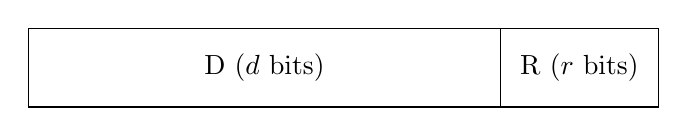
\begin{tikzpicture}
        \draw (0,0) rectangle (8,1);
        \draw (6,0) -- (6,1);
        \draw (3,0.5) node {D ($ d $ bits)};
        \draw (7,0.5) node {R ($ r $ bits)};
    \end{tikzpicture}
    \caption{CRC}
\end{figure}

\vspace{0.5cm}

发送方需要构造的长度为$ d + r $位的序列可以通过将数据$ D $左移$ r $位,并加上$ R $得到。由于得到的$ d + r $位序列能够被$ G $整除,即为$ G $的整数倍。

\vspace{-1cm}

\begin{align*}
    D \cdot 2^r\ \text{XOR}\ R = nG
\end{align*}

等式两边同时XOR $ R $,得到:

\vspace{-1cm}

\begin{align*}
    D \cdot 2^r = nG\ \text{XOR}\ R
\end{align*}

$ R $为$ D \cdot 2^r $除以$ G $的余数:

\vspace{-1cm}

\begin{align*}
    R = \text{remainder}\left[{D \cdot 2^r} \over G\right]
\end{align*}

